\chapter{Cost-Benefit Analysis}
\section{What is cost-benefit analysis?}
\begin{quote}
  ``Assessing costs and benefits across all affected groups or places matters because even a proposal with a relatively low public sector cost such as new regulation, may have significant effects on specific groups in society, places or business''
\end{quote}
\begin{itemize}
  \item A cost-benefit analysis is the process used to measure the benefits of a decision or taking action relative to the associated costs
  \item If benefits $>$ costs, the decision or action is a good one to take
  \item If costs $>$ benefits, the proposed action or decision should be reconsidered
  \item Cost benefit analysis can also be used to compare alternate decisions or actions
\end{itemize}
Both costs and benefits are required to be expressed in monetary terms, accounting for the time value of money. Costs may be categorised as:
\begin{itemize}
  \item Direct - e.g. labour costs, manufacturing costs, material costs
  \item Indirect - e.g. utilities, rent
  \item Intangible - e.g. reduced productivity because of a new process
  \item Opportunity - lost benefits (opportunities) when pursuing one strategy over another
\end{itemize}
Benefits may be categorised as:
\begin{itemize}
  \item Direct - e.g. increased revenue and sales
  \item Indirect - e.g. increased consumer interest
  \item Intangible - e.g. improved employee morale
  \item Competitive - e.g. being an industry leader
\end{itemize}
\section{The Benefit-Cost Ratio method}
The Benefit-Cost Ratio (BCR) is defined as the ratio of the equivalent value of benefits to the equivalent value of costs. The equivalent-value measure can be:
\begin{itemize}
  \item Annual value (AV)
  \item Present value (PV)
  \item Future value (FV)
\end{itemize}
The BCR method has been the accepted procedure for making decisions and comparing projects in the public sector for many decades.
\begin{quote}
  if BCR $\geq$ 1, the project is acceptable
\end{quote}
Several different formulations of the BCR method have been developed. We examine two formulations of the BCR method that are commonly used by government agencies:
\begin{itemize}
  \item Conventional BCR method
  \item Modified BCR method
\end{itemize}
Both formulations will lead to identical project acceptability decisions (i.e. BCR $\geq$ 1 or BCR $<$ 1).
\subsection{Conventional BCR method}
Present value (PV) formulation:
\begin{gather}
  BCR_{PV} = \dfrac{PV_{benefits}}{PV_{costs}}\\
  BCR_{PV} = \dfrac{PV_{benefits}}{I- PV_{MV}+PV_{O\&M}}
\end{gather}
Annual value (AV) formulation:
\begin{gather}
  BCR_{AV} = \dfrac{AV_{benefits}}{AV_{costs}}\\
  BCR_{AV} = \dfrac{AV_{benefits}}{CR + AV_{O\&M}}
\end{gather}
Both ratios lead to identical numerical results. Where:
\begin{itemize}
  \item $I$ is initial investment in the proposed project
  \item $MV$ is market value at the end of useful life
  \item $O\&M$ is operating and maintenance costs
  \item $CR$ is capital-recovery amount (i.e. equivalent cost of $I$, including an allowance for market or salvage value)
\end{itemize}
\subsection{Modified BCR method}
Present value (PV) formulation:
\begin{gather}
  BCR_{PV} = \dfrac{PV_{benefits}}{PV_{costs}}\\
  BCR_{PV} = \dfrac{PV_{benefits} - PV_{O\&M}}{I - PV_{MV}}
\end{gather}
Annual value (AV) formulation:
\begin{gather}
  BCR_{AV} = \dfrac{AV_{benefits}}{AV_{costs}}\\
  BCR_{AV} = \dfrac{AV_{benefits}-AV_{O\&M}}{CR}
\end{gather}
Both ratios lead to identical numerical results.
\subsection{Conventional and modified BCRs}
Remember the formula for PV:
\begin{gather}
  PV = \dfrac{FV}{(1+i)^n}
\end{gather}
Present value (PV) of a future value (FV) in $n$ years, for an interest rate $i$.
Remember the formula for AV:
\begin{gather}
  AV = PV\dfrac{i(1+i)^n}{(1+i)^n - 1}
\end{gather}
Value of a series of uniform (annual) receipts (AV) that occur at the end of periods (years) 1 to $n$, given their present value (PV) and an interest rate $i$.
\subsection{What value of i to use?}
There are three main considerations when it comes to what interest rate to use for engineering economy studies of public-sector projects:
\begin{itemize}
  \item the interest rate on borrowed capital
  \item The opportunity cost of capital to the government agency
  \item The opportunity cost of capital to the taxpayers
\end{itemize}
\subsection{Why do conventional and modified BCRs lead to the same decision?}
Conventional BCR formulation:
\begin{gather}
  BCR_V = \frac{V_{benefits}}{I - V_{MV}+V_{O\& M}} = \frac{B}{C}
\end{gather}
Where subscript $V$ denotes either PV or AV. Modified BCR formulation:
\begin{gather}
  BCR_V = \frac{V_{benefits} \textcolor{red}{-V_{O\&M}}}{I - V_{MV} + V_{O\&M} \textcolor{red}{-V_{O\&M}}} = \frac{B\textcolor{red}{-X}}{C\textcolor{red}{-X}}
\end{gather}
Both the numerator and denominator differ by the same constant.
\begin{gather}
  \textcolor{red}{\frac{B}{C>1}}\rightarrow B > C \rightarrow B - X > C - X \rightarrow \textcolor{red}{\frac{B-X}{C-X}>1}
\end{gather}
leading to the same decision.
\subsection{Example 1}
The Greater London Authority is considering extending the runways of Stansted Airport so that larger commercial airplanes can use the facility. The land necessary for the runway extension is currently a farmland that can be purchased for \pounds 350,000. Construction costs for the runway extension are projected to be \pounds 600,000, and the additional annual maintenance costs for the extension are estimated to be \pounds 22,500. If the runways are extended, a small terminal will be constructed at a cost of \pounds 250,000. The annual operating and maintenance costs for the terminal are estimated at \pounds 75,000. Finally, the projected increase in flights will require the addition of two air traffic controllers at an annual cost of \pounds 100,000. Annual benefits of the runway extension have been estimated as follows:
\begin{table}
  \centering
  \begin{tabular}{@{}ll@{}}
    \toprule
    \textbf{Description}                            & \textbf{Annual benefit}  \\
    \midrule
    Leasing fee receipts from airlines              & \pounds 325,000          \\
    Passenger airport tax receipts                  & \pounds 65,000           \\
    Convenience benefit for residents near Stansted & \pounds 50,000           \\
    Additional tourism money for London             & \pounds 50,000           \\
    \midrule
    \textbf{Total}                                  & \textbf{\pounds 490,000} \\
    \bottomrule
  \end{tabular}
  \caption{Example 1.}
\end{table}
Apply the BCR method with a study of 20 years and a MARR of 10\% per year to determine whether the runways at Stansted airport should be extended.

Information provided:
\begin{gather}
  i = 0.1\\
  n = 20\, \textrm{years}\\
  I = \pounds 350000 + \pounds 600000 + \pounds 250000 = \pounds 1200000\\
  AV_{benefits} = \pounds 490000\\
  PV_{MV} = AV_{MV} = \pounds 0\\
  AV_{O\&M} = \pounds 22500 + \pounds 75000 + \pounds 100000 = \pounds 197500
\end{gather}
First, we need to determine PVs and AVs using:
\begin{gather}
  PV = AV\frac{\left(1+i\right)^n - 1}{i\left(1 + i\right)^n}\\
  AV = PV\frac{i\left(1+i\right)^n}{\left(1+i\right)^n - 1}
\end{gather}
\begin{gather}
  PV_{benefits} = \pounds 4171646\\
  PV_{O\&M} = \pounds 1681429\\
  AV_I = CR = \pounds 140951
\end{gather}
Conventional BCRs:
\begin{gather}
  BCR_{PV} = \frac{PV_{benefits}}{I - PV_{MV}+PV_{O\&M}} = 1.448\\
  BCR_{AV} = \frac{AV_{benefits}}{CR + AV_{O\&M}} = 1.448
\end{gather}
Modified BCRs:
\begin{gather}
  BCR_{PV} = \frac{PV_{benefits} - PV_{O\&M}}{I - PV_{O\&M}} = 2.075\\
  BCR_{AV} = \frac{AV_{benefits}- AV_{O\&M}}{CR} = 2.075
\end{gather}
BCR $\geq$ 1 in all cases, so runway should be extended.
\subsection{Issues of concern using BCRs}
\begin{itemize}
  \item The treatment of disbenefits
        \begin{itemize}
          \item Negative consequences to the public resulting from the implementation of a public sector project
        \end{itemize}
  \item The treatment of certain cash flows as additional benefits or reduced costs
\end{itemize}
\subsection{Treatment of disbenefits}
Disbenefits can be incorporated in BCR calculations by:
\begin{itemize}
  \item Reducing benefits accordingly (traditional approach) or
  \item Increasing costs accordingly
\end{itemize}
How do these approaches affect the BCR? How do these approaches affect the final decision?
\subsection{Example 2}
Refer back to Example 1. Suppose that there are disbenefits associated with the runway extension project. Specifically, the increased noise level from commercial jet traffic will be a serious nuisance to homeowners living along the approach path Stansted Airport. The annual disbenefit to these citizens is estimated to be \pounds 100,000.

Reapply the conventional BCR method, with equivalent annual worth, to determine whether this disbenefit affects your recommendation on the desirability of this project.

Disbenefit treated as a reduced benefit:
\begin{gather}
  BCR_{AV} = \frac{AV_{benefits}-100000}{CR + AV_{O\&M}} = 1.152
\end{gather}
Disbenefit treated as an increased cost:
\begin{gather}
  BCR_{AV} = \frac{AV_{benefits}}{CR + AV_{O\&M}+100000} = 1.118
\end{gather}
BCR $\geq$ 1 in both cases, so runway should be extended. The treatment of disbenefits affects the magnitude of the BCR, but not the decision.
\subsection{Treatment of certain cash flows}
Certain cash flows can be incorporated in BCR calculations by:
\begin{enumerate}
  \item Increasing benefits accordingly
  \item Reducing costs accordingly
\end{enumerate}
How do these approaches affect the BCR? How do these approaches affect the final decision?
\subsection{Example 3}
Transport for London is considering upgrading an ageing bridge across the Thames. The existing two-lane bridge is expensive to maintain and creates a traffic bottleneck because the road is four lanes wide on either side of the bridge. The new bridge can be constructed at a cost of \pounds 300,000, and estimated annual maintenance costs are \pounds 10,000. The existing bridge has annual maintenance costs of \pounds 18,500. The annual benefit of the new four-lane bridge to motorists, due to the removal of the traffic bottleneck, has been estimated to be \pounds 25,000.

Conduct a cost-benefit analysis based on equivalent annual worth, using a MARR of 8\% and a study period of 25 years, to determine whether the new bridge should be constructed.

Information provided:
\begin{gather}
  i = 0.08\\
  n = 25\, \textrm{years}\\
  I = \pounds 300000\\
  AV_{benefits} = \pounds 25000\\
  PV_{MV} = AV_{MV} = \pounds 0\\
  AV_{O\&M} = \pounds 10000 - \pounds 18500 = \textcolor{red}{-\pounds 8500}
\end{gather}
Cost is negative because it represents a reduction with respect to the current cost.

Required information:
\begin{gather}
  AV_I = CR = \pounds 28104
\end{gather}
Reduced cost treated as a reduced cost (conventional BCR approach):
\begin{gather}
  BCR_{AV} = \frac{BCR_{AV}}{CR + AV_{O\&M}} = 1.275
\end{gather}
Reduced cost treated as an increased benefit (modified BCR approach):
\begin{gather}
  BCR_{AV} = \frac{AV_{benefits} - AV_{O\&M}}{CR} = 1.192
\end{gather}
BCR $\geq$ 1 in both cases, so bridge should be constructed. The classification of the cash-flow items affects the magnitude of the BCR, but not the decision.
\subsection{Treatment of disbenefits/certain cash flows}
Arbitrary decisions on the classification of benefits and costs has no bearing on project acceptability because if X is classified as an added benefit:
\begin{gather}
  BCR = \frac{B \textcolor{red}{+ X }}{C}
\end{gather}
and
\begin{gather}
  BCR > 1 \rightarrow B + X > C \rightarrow B > C - X \rightarrow \frac{B}{C \textcolor{red}{- X}} > 1
\end{gather}
leading to the same decision.
\section{Evaluating independent projects using the BCR method}
\subsection{What are independent projects?}
Independent projects are categorised as groupings of projects for which the choice to select any particular project in the group is \textbf{independent} of choices regarding all other projects within the group.

It is therefore acceptable to select:
\begin{enumerate}
  \item None of the projects
  \item A combination of the projects
  \item All of the projects
\end{enumerate}
Formal comparisons of independent projects is unnecessary. The only criterion for selecting each independent project is BCR $\geq$ 1.
\subsection{Example 4}
Uncontrolled water flow has increased flow conditions along a river. You have independent options to alleviate the problem of building a reservoir and/or improving the channel. Relevant information is as follows:
\begin{table}[H]
  \centering
  \begin{tabular}{@{}lll@{}}
    \toprule
                     & Reservoir construction & Channel improvement \\
    \midrule
    $CR + AV_{O\&M}$ & \pounds 1,642,200      & \pounds 1,815,100   \\
    $AV_{benefits}$  & \pounds 1,742,200      & \pounds 2,856,300   \\
    \bottomrule
  \end{tabular}
  \caption{Example 4 information.}
\end{table}
Conduct a cost-benefit analysis using the conventional BCR method and equivalent annual worth to determine the best course of action.

Reservoir construction:
\begin{gather}
  BCR_{AV} = \frac{AV_{benefits}}{CR + AV_{O\&M}} = 1.061
\end{gather}
Channel improvement:
\begin{gather}
  BCR_{AV} = \frac{AV_{benefits}}{CR + AV_{O\&M}} = 1.574
\end{gather}
BCR $\geq$ 1 in both cases, so both options should be pursued (the fact that the channel improvement has a higher BCR is irrelevant).
\section{Evaluating mutually exclusive projects using the BCR method}
\subsection{What are mutually exclusive projects}
Mutually exclusive projects are a group of projects from which, \textbf{at most, one project may be selected.} Each mutually exclusive project can be viewed as a feasible design alternative. Because the BCR method provides a ratio of benefits to costs rather than a direct measure of a project's profit potential, \textbf{selecting the project that maximises the BCR does not guarantee that the best project is selected.}
\subsection{Procedure for evaluating mutually exclusive projects}
\begin{enumerate}
  \item Calculate equivalent value (PV, AV or FV) of costs for each mutually exclusive project
  \item Rank-order mutually exclusive projects by increasing equivalent value of costs (note: the rank-order will be the same for all equivalent value types)
  \item Calculate the BCR for the project with the lowest equivalent cost ($BCR_L$)
        \begin{itemize}
          \item If $BCR_L \geq 1 \rightarrow$ baseline = project with the lowest equivalent cost
          \item Else $\rightarrow$ baseline = ``do-nothing''
        \end{itemize}
  \item Follow the flow chart in Figure \ref{fig:EMEFC}
\end{enumerate}
\begin{figure}[H]
  \centering
  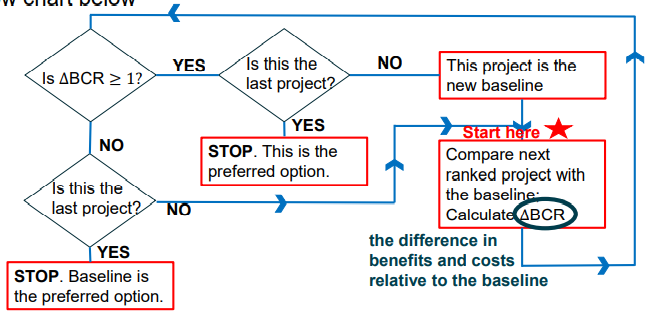
\includegraphics[width = 0.9\textwidth]{./img/figure25.png}
  \caption{Flow chart for evaluating mutually exclusive projects}
  \label{fig:EMEFC}
\end{figure}
\subsection{Example 5}
Three mutually exclusive public-works projects are currently under consideration. Their respective costs and benefits are included in the table that follows. Each of the projects has a useful life of 50 years, and MARR is 10\% per year.
\begin{table}[H]
  \centering
  \begin{tabular}{@{}llll@{}}
    \toprule
                       & Project A         & Project B          & Project C          \\
    \midrule
    Capital investment & \pounds 8,500,000 & \pounds 10,000,000 & \pounds 12,000,000 \\
    Annual O\&M costs  & \pounds 750,000   & \pounds 725,000    & \pounds 700,000    \\
    Market value       & \pounds 1,250,000 & \pounds 1,750,000  & \pounds 2,000,000  \\
    Annual benefit     & \pounds 2,150,000 & \pounds 2,265,000  & \pounds 2,500,000  \\
    \bottomrule
  \end{tabular}
  \caption{Example 5 information.}
\end{table}
Which, if any of these projects, should be selected?

Information provided and required information:
\begin{gather}
  i = 0.1\\
  n = 50\, \textrm{years}
\end{gather}
Step 1: convert to PV.
\begin{table}[H]
  \centering
  \begin{tabular}{@{}llll@{}}
    \toprule
                    & Project A          & Project B          & Project C          \\
    \midrule
    I               & \pounds 8,500,000  & \pounds 10,000,000 & \pounds 12,000,000 \\
    $PV_{O\&M}$     & \pounds 7,436,111  & \pounds 7,188,241  & \pounds 6,940,370  \\
    $PV_{MV}$       & \pounds 10,648     & \pounds 14,907     & \pounds 17,037     \\
    $PV_{costs}$    & \pounds 15,925,463 & \pounds 17,173,333 & \pounds 18,923,333 \\
    $PV_{benefits}$ & \pounds 21,316,851 & \pounds 22,457,055 & \pounds 24,787,036 \\
    \bottomrule
  \end{tabular}
  \caption{Example 5 required information.}
\end{table}
Step 2
\begin{gather}
  BCR_A = \frac{21316851}{15925463} = 1.339 \geq 1 \rightarrow\, \textrm{Project A is the baseline}
\end{gather}
Step 3: establish baseline.

Step 4:
\begin{gather}
  \Delta BCR_{B} = \frac{22457055-21316851}{17173333-15925463} = 0.914 < 1 \rightarrow\, \textrm{Project A is still the baseline}
\end{gather}
Proceed to Project C
\begin{gather}
  \Delta BCR_{C} = \frac{24787036-21316851}{18923333-15925463} = 1.158 \geq 1 \rightarrow\, \textrm{Project C is the preferred option}
\end{gather}
\subsection{Mutually exclusive projects with unequal lives}
It is not uncommon for public projects to have different useful lives. How can we conduct BCR analyses in these cases? In these cases, annual values (AVs) should be used to conduct incremental cost-benefit analyses.
\subsection{Example 6}
Two mutually exclusive alternative public-works projects are under consideration. Their respective costs and benefits are included in the table that follows. Project A has an anticipated life of 35 years, and the useful life of Project B has been estimated to be 25 years. The effect of inflation is negligible.
\begin{table}[H]
  \centering
  \begin{tabular}{@{}lll@{}}
    \toprule
                       & Project A       & Project B       \\
    \midrule
    Capital investment & \pounds 750,000 & \pounds 625,000 \\
    Annual O\&M costs  & \pounds 120,000 & \pounds 110,000 \\
    Annual benefit     & \pounds 245,000 & \pounds 230,000 \\
    \bottomrule
  \end{tabular}
  \caption{Example 6 information.}
\end{table}
If the MARR is 9\% per year, which, if either, of these projects should be selected?

Information provided and required information:
\begin{gather}
  i = 0.09\\
  n = 35 \textrm{ or } 25\, \textrm{years}
\end{gather}
Step 1: convert to AV.
\begin{table}[H]
  \centering
  \begin{tabular}{@{}lll@{}}
    \toprule
                    & Project A       & Project B       \\
    \midrule
    $AV_I$          & \pounds 70,977  & \pounds 63,629  \\
    $AV_{O\&M}$     & \pounds 120,000 & \pounds 110,000 \\
    $AV_{MV}$       & \pounds 0       & \pounds 0       \\
    $AV_{costs}$    & \pounds 190,977 & \pounds 173,629 \\
    $AV_{benefits}$ & \pounds 245,000 & \pounds 230,000 \\
    \bottomrule
  \end{tabular}
  \caption{Example 6 required information.}
\end{table}
Step 2:
\begin{gather}
  BCR_B = \frac{230000}{173629} = 1.325 \geq 1 \rightarrow \, \textrm{Project B is the baseline}
\end{gather}
Step 3: establish baseline.

Step 4:
\begin{gather}
  \Delta BCR_A = \frac{245000 - 230000}{190977-173629}=0.865<1\rightarrow\,\textrm{Project B is the preferred option}
\end{gather}